\documentclass[fr]{../../../eplsummary}

\usepackage{../../../eplunits}

\hypertitle{Internal combustion engines}{8}{MECA}{2220}
{Étudiants MECA 2017}
{Hervé Jeanmart}

\paragraph{Note} Synthèse des questions de l'examen oral.

\section{Thermodynamique et description fondamentale}

\subsection{Quel est l'influence de la richesse (et donc de la température!) sur le rendement thermodynamique ?}
Dans le modèle de Beau de Rochas (BDR), on peut exprimer le rendement $\eta_{th} = 1 - \frac{1}{\tau^{\gamma-1}} $.

Cette formule ne tient pas compte de l'évolution des chaleurs massiques des différents composés avec la température. En incluant ce phénomène, le rendement suit alors l'évolution montrée à la Figure \ref{rendement_BDR_fig}, et l'exposant $\gamma-1$ peut être remplacé par $x$ de la régression linéaire de l'Eq. \ref{rendement_BDR_x}. On remarque donc que le rendement $\eta_{th}$ est d'autant plus élévé que $\phi$ est faible et que $\tau$ est élévé. Notons tout de même que $\phi$ ne peut être trop faible, car il faut s'assurer que la combustion ait bien toujours lieux.
\begin{equation}
x = 0.277 + 0.06 (1-\phi + (1-0.1\tau^{0.5})\cdot (1-\phi)^{2.5})
\label{rendement_BDR_x}
\end{equation}

L'influence de la température sur le rendement thermodynamique peut également être vue sous un autre angle. En effet, ce dernier est donné par 
\[ \eta_{ti} = 1-\epsilon_E - \epsilon_P \]
C'est pourquoi, la température a un effet néfaste puisque vient augmenter les pertes de chaleurs pariétales.
\begin{figure} [H]
  \centering
  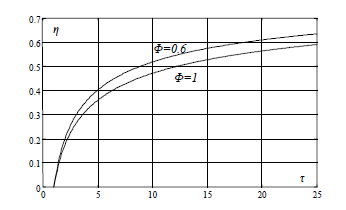
\includegraphics{img/Chap1_Q1.PNG}
  \caption{rendement en fonction de $\phi$ et $\tau$}
  \label{rendement_BDR_fig}
\end{figure}

\subsection{Expliquer pourquoi le taux de compression et gamma augmentent le rendement thermodynamique ? Pourquoi quand gamma augmente, le rendement augmente? (Physiquement)}
\label{chap1Q2}
Comme montré plus haut, $\eta_{th}$ du cycle de Beau de Rochas augmente avec $\gamma$ et $\tau$. Quelle interprétation physique donner à cela?

Pour $\tau$ c'est assez direct, puisque l'apport de chaleur survient dans un état plus éloigné de l'état initial, et produit donc plus de travail (cf. aire entre les courbes).

Pour $\gamma$, rappelons les expressions des capacités calorifiques en fonction de $R^*$ et $\gamma$:
\begin{eqnarray*}
  C_v	&=& \cfrac{R^*}{\gamma-1}\\
  C_p	&=& \cfrac{\gamma R^*}{\gamma-1}\\
  \cfrac{\partial C_v}{\partial\gamma}	&=& \cfrac{-R^*}{(\gamma-1)^2} <0\\
  \cfrac{\partial C_p}{\partial\gamma}	&=& \cfrac{-R^*}{(\gamma-1)^2} <0
\end{eqnarray*}
Donc $C_p$ et $C_v$ diminuent avec $\gamma$ qui augmente, et donc la quantité de chaleur stockée dans les gaz d'échappement diminue (pour une même température de ces gaz). C'est pourquoi le rendement augmente (puisque $\epsilon_E$ plus faible).


\subsection{Quel est l'intérêt de Sabathé par rapport à Beau de Rochas et à Diesel?}

Les cycles de Beau de Rochas et Diesel sont des cycles similaires qui présentent 4 phases dont trois les mêmes et une différente (la deuxième).
\begin{itemize}
    \item $ 1 \rightarrow 2 $ : Compression isentropique
    \item $ 2 \rightarrow 3 $: Réchauffement isochore/isobare pour le cas BDR/Diesel
    \item $ 3 \rightarrow 4 $: Détente isentropique
    \item $ 4 \rightarrow 1 $: Refroidissement isochore
\end{itemize}

\begin{figure}[ht] 
  \begin{minipage}[b]{0.33\linewidth}
    \begin{center}
        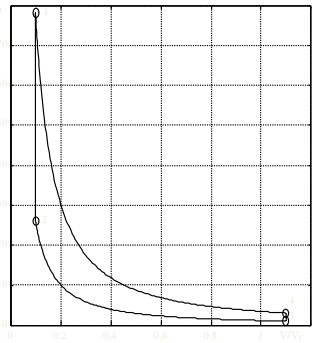
\includegraphics[width = \textwidth]{img/Chap1_Q4_BDR.PNG} 
        \caption{BDR}
    \end{center}
  \end{minipage} 
  \begin{minipage}[b]{0.33\linewidth}
    \begin{center}
        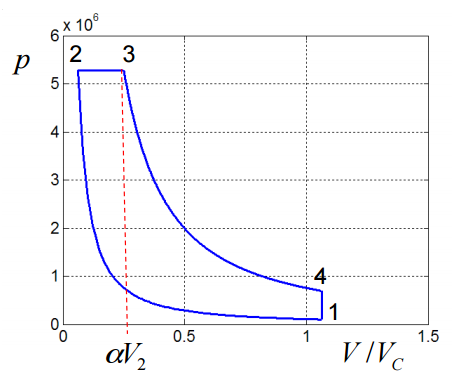
\includegraphics[width = \textwidth]{img/Chap1_Q4_Diesel.PNG} 
        \caption{Diesel}
    \end{center}
  \end{minipage}  
  \begin{minipage}[b]{0.33\linewidth}
    \begin{center}
        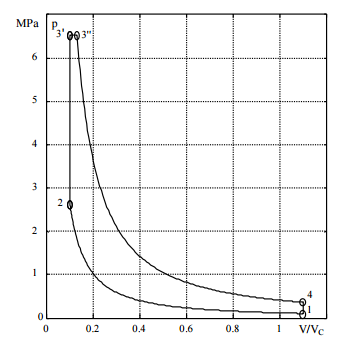
\includegraphics[width = \textwidth]{img/Chap1_Q4_Sabathe.PNG} 
        \caption{Sabathé}
    \end{center}
  \end{minipage}  
\end{figure}

Le cycle de Sabathé quant à lui est un mix entre les 2, il enchaine les 2 phases l'une à la suite de l'autre : 
\begin{itemize}
    \item $ 2 \rightarrow 3' $: Réchauffement isochore
    \item $ 3' \rightarrow 3'' $: Réchauffement isobare
\end{itemize}


Deux paramètres importants apparaissent alors dans l'expression du cycle de Sabathé :
\begin{center}
  $\beta = \cfrac{T_{3'}}{T_{2}}$ et $ \chi = \cfrac{T_{3''}}{T_{3'}} $
\end{center}

Avec les 2 cas limites, Sabathé$\rightarrow$BDR si $\chi=1$ et Sabathé$\rightarrow$Diesel si $\beta=1$

L'intérêt de ce dernier cycle est de mieux épouser l'évolution du couple p-V au cours du cycle réel, et donc de mieux estimer le rendement du cycle grâce aux paramètres $\beta$ et $\chi$ (l'effet est facilement compréhensible si on regarde l'aire dans la courbe du cycle). Le rendement est alors multiplié par le facteur de troncature suivant :
\begin{center}
  $\eta = 1 - \cfrac{1}{\tau^{\gamma-1}}\cfrac{\beta \chi^{\gamma}-1}{\beta -1 + \gamma \beta (\chi - 1)}$
\end{center}

Néanmoins le cycle de Sabathé est très peu utilisé car le facteur de troncature est proche de 1 (+/- 0.95), ce qui rend la démarche très couteuse en temps, en coûts et en calcul par rapport à ce qu'on y gagne.


\subsection{Pourquoi échauffement est isobare alors que c'est encore moins faisable que de faire un échauffement isochore ?}
La combustion en moteur CI est plus lente qu'en moteur SI. Cela peut s'expliquer par les différentes phases de la combustion (délais à l'auto-ignition - combustion lente - combustion rapide, cf. syllabus p104). Cette lenteur explique par ailleurs la différence de vitesses de rotation entre moteur SI et CI. La combustion est alors étalée sur un plus grand CAD, et vient donc maintenir un certain temps la pression à une valeur quasi-constante, alors même que l'expansion est en cours. C'est pourquoi, un modèle à apport de chaleur isobare peut être intéressant pour modéliser certains types de moteurs (en l'occurence CI).


\section{Aspects thermiques et PMI}

\subsection{Pertes pariétales : origine, ordre de grandeur, paramètres d'influence}
\paragraph{Origine} $\Delta T$ entre l'intérieur du cylindre et la paroi. La T des parois ne varie pas très fort à cause de l'inertie thermique. Les pertes à travers la paroi diminue la chaleur disponible pour fournir du travail. 

\paragraph{Ordre de grandeur} $\epsilon_p$ varie de 10\% à 20\%. Mode principal est de type convectif, avec éventuellement une partie par rayonnement en CI (jusque 25\%).

\paragraph{Paramètres d'influence} Sur base de 
\begin{itemize}
    \item La corrélation de Colburn (pour le nombre de Nüsselt $Nu$)    
    \item Différentes grandeurs liées à la mécanique des fluides et à la thermodynamique (dont $Pr$, cf. syllabus p. 27).
    \item $C\approx D$
\end{itemize}
Il est possible d'obtenir l'expression suivante (cf. syllabus Eq. 2.2b p. 28):
\[ \epsilon_P \approx \SI{0.015}{}(ruD)^{-0.2}(\tau^{0.8} + 3\tau^{-0.4}) \]
On obtiens donc une dépendance envers $r$, $u$ et $D$ qui nous pousse à les maximiser, et envers $\tau$ qui nous pousse à le minimiser.




\subsection{Quelle est l'origine du rayonnement dans un moteur diesel ? Quel est l'effet sur le rendement si on suppose les parois adiabatiques ?}
La combustion en moteur CI s'opère via la auto-ignition, et donc la création puis diffusion de radicaux carbonés lourds. Ce caractère diffusionnel de la flamme entraine une plus grande émissivité, et donc un transfert de chaleur par rayonnement. Sous l'hypothèse de parois adiabatiques ($q = 0$), cela ne doit pas avoir d'impact sur le rendement car cette énergie ne peut s'échapper du cylindre. Au contraire, cela devrait même avoir un impact positif, le rayonnement pouvant entraîner la formation de radicaux dans les zones plus froides (ie. proche des parois) et donc favoriser l'auto-ignition.

Des parois adiabatiques peuvent donc mener à une plus grand rendement thermodynamique $\eta_{ti}$ ($\epsilon_P = 0$), mais également un plus grand rendement de combustion $\eta_c$ (moins d'imbrulés, car meilleure propagation de la flamme proche des parois).

\subsection{Lien entre pertes pariétales et pertes à l'échappement ?}
Les différentes aires représentées sur le diagramme TS du cycle de la Figure \ref{chap2_Q3_TS} peuvent etre interprétées comme suit:
\begin{itemize}
    \item Chaleur dégagée par la combustion $Q_{c}=A+B+C+D$
    \item Travail thermodynamique $W_{i}=A$
    \item Pertes pariétales de chaleur : $Q_{P} = B+D$
    \item Pertes de chaleur à l'échappement: $Q_{E} = C$
\end{itemize}

Du coup, pour un même apport de chaleur par combustion $Q_c$, si $Q_P$ diminue $Q_E$ augmente. Ce constat graphique est par ailleurs appuyé par l'expression du coefficient de pertes de chaleur à l'échappement (en reprenant la régression linéaire du cycle de Beau de Rochas avec chaleurs massiques moyennes):
\[\epsilon_E = \frac{1}{\tau^x}-\epsilon_{P}\frac{2}{\tau^{x}+1}\]
\begin{figure} [H]
  \centering
  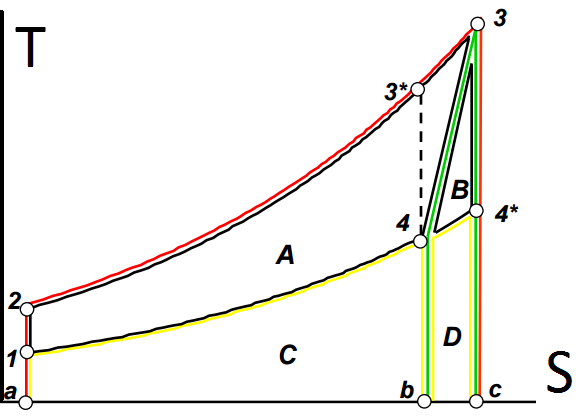
\includegraphics[scale=0.3]{img/Chap2_Q3.PNG}
  \caption{Diagrammme T-S du cycle moteur.}
  \label{chap2_Q3_TS}
\end{figure}


\subsection{Que représente le \texorpdfstring{$\frac{1}{\tau^x}$}{1/tau x} dans la formule des pertes à l'échappement ?}
$$\epsilon_E = \cfrac{1}{\tau^x} - \epsilon_P\cfrac{2}{\tau^x+1}$$
En reprenant le cycle de Beau de Rochas, obtenue en considérant des chaleurs massiques variables avec la température (et donc non constantes), son rendement thermique est exprimé par 
\[ \eta_{ti} = 1-\cfrac{1}{\tau^x} \]
Le terme $1/\tau^x$ représente donc les pertes totales de chaleurs du cycle thermodynamique en l'absence de pertes pariétales. Elles sont alors uniquement constituées de pertes à l'échappement, fixées par les caractéristiques du cycle ainsi que l'apport de chaleur (paramètres $\tau$ et $x$).


\subsection{Quel type de moteur essence utilise t-on pour diminuer les pertes pariétales ?}
\textbf{Injection directe}: moins de surfaces de parois par rapport à l'injection indirecte.

\textbf{Charge stratifiée}: à faible charge, on concentre le fuel près de la bougie pour obtenir une richesse locale qui soit suffisament élevée pour assurer la combustion. La combustion est donc concentrée loins des parois, et limite le transfert de chaleur.

\subsection{Influence de la richesse sur pmi ?}
\label{Chap2Q6}
\begin{eqnarray*}
 pmi	&=& \frac{W_{i}-W_{p}}{V_c}\\
	&=& \eta_{ti}\eta_{c}\cfrac{m_{c}PCI}{V_c} - (p_{e}-p_{a})\\
	&=& \eta_{ti}\eta_{c}\cfrac{\phi m_aPCI}{m_{a1}V_c} - (p_{e}-p_{a})
\end{eqnarray*}

Dans le cas de carburants liquides, nous avons:
\begin{eqnarray*}
 m_a	&=& r\rho_0V_c\\
 pmi	&=& \eta_{ti}\eta_{c}r\cfrac{\phi PCI}{m_{a1}}\rho_0 - (p_{e}-p_{a})
\end{eqnarray*}

Et pour les carburants gazeux:
\begin{eqnarray*}
 m_a	&=& r\cfrac{V_{a1}}{V_{a1}+\phi}\rho_0V_c\\
 pmi	&=& \eta_{ti}\eta_{c}r\cfrac{V_{a1}}{V_{a1}+\phi}\cdot\cfrac{\phi PCI}{m_{a1}}\rho_0 - (p_{e}-p_{a})
\end{eqnarray*}

On observe donc dans les deux cas une influence favorable de $\phi$ sur $pmi$, même dans le cas de la plupart des carburants gazeux car $\phi<<V_{a1}$ (sauf pour le gazogène, $V_{a1}>6$, cf. syllabus p. 69).


\subsection{PMI : définition, paramètres d'influence, lien avec les autres paramètres. Pourquoi l'utilise t-on comme référence pour comparer des moteurs ?}
Pression moyenne indiquée, définie comme $pmi = W_{ind}/V_c$. Le travail indiqué $W_{ind}$ prend en compte le rendement de combustion, rendement du cycle thermodynamique (pertes de chaleur) ainsi que les pertes par pompage. Seules les pertes mécaniques ne sont pas considérées. Rapporté à la cylindrée, cela permet de comparer les moteurs en faisant abstraction de leur taille, de leur puissance ou du combustible qu'ils brulent.

Paramètres d'influence: cf. expression de $pmi$ à la Question \ref{Chap2Q6}, ou p. 34 du syllabus.


\subsection{Signification de la température d'échappement \texorpdfstring{$T_5$}{T5} et de celle en fin de cycle \texorpdfstring{$T_4$}{T4}? Comment calculer \texorpdfstring{$T_{5}$}{T5} à partir de \texorpdfstring{$T_4$}{T4}?}
\label{Chap2Q8}
La pression $p_4$ en fin de cycle est différente de la pression atmosphérique. La température $T_5$ est donc celle des gaz d'échappement une fois ramenés à la pression atmosphérique. L'expansion à effectuer n'est cependant pas parfaitement adiabatique, et induit donc un coefficient de pertes pariétales de chaleur à l'échappement $\epsilon_{PE}$. 

$T_5$ peut etre obtenue en
\begin{itemize}
 \item Calculant une température d'échappement adiabatique $T_5^*$. Pour ce faire, $pV^\gamma=C$ n'est d'aucune utilité, car système ouvert donc $V=?$. Nous devons plutot égaler les chaleurs dégagées par l'échappement des états 4 et $5^*$ puisque la transformation $4-5^*$ est adiabatique. Cela se fait en opérant le bilan énergétique suivant (avec l'état 1 comme référence):
 \begin{eqnarray*}
  Q_{5^*-1} 	&=& Q_{4-1}\\
  q_{5^*-1}	&=& dH - Vdp = C_p dT \text{ car transformation isobare}\\
  q_{4-1}	&=& dU + pdV = C_v dT \text{ car transformation isochore}
 \end{eqnarray*}
 L'expression finale de $t_5^* = T_5^* - \SI{273.15}{K}$ est donnée à l'Eq. (2.18) p. 38 du syllabus, ou CM4 slide 14.
 
 \item Opérant un bilan énergétique des pertes pariétales de chaleurs à l'échappement, cf CM4 slide 15 ou syllabus p. 39 Eq. (2.19).
\end{itemize}


\subsection{Comment calcule-t-on la température à l'échappement \texorpdfstring{$T_5^*$}?}
Cf. Question \ref{Chap2Q8}. Sans se compliquer la tache à utiliser précisément les chaleurs massiques moyennes des différents composés, il est également possible d'obtenir directement à partir des égalités présentées ci-dessus:
\begin{eqnarray*}
 Q_{5^*-1}	&=& Q_{4-1}\\
 C_p(T_5^*-T_1)	&=& C_v(T_4-T1)\\
 T_5^*		&=& T_1 + \cfrac{T_4-T_1}{\gamma}
\end{eqnarray*}

\subsection{Qu'est ce qu'un turbocompresseur ? Utilité dans les moteurs ?}
\label{Chap2Q10}
Le concept de base est illustré à la Figure \ref{Chap2_turbo}: cela consiste en l'utilisation d'une turbine permettant de récupérer une partie de l'énergie d'expansion des gaz d'échappement, pour comprimer l'air à l'admission et donc augmenter le remplissage $r$ (pour lui donner des valeurs supérieures à 1, typiquement aux alentours de 2-3).

L'augmentation du remplissage a pour intéret d'augment $pmi$ pour un même moteur, et permet donc d'atteindre des plus grandes densités de puissance. Elle n'a pas d'influence directe sur le rendement indiqué, mais permet tout de même de l'augmenter indirectement, à travers (cf. syllabus p. 43):
\begin{itemize}
 \item Diminution de $\epsilon_P$ (car plus grande énergie de combustion $Q_I$ pour la même surface de parois).
 \item Amélioration du rendement de combustion $\eta_c$ par limitation du niveaux d'imbrulés (obtenue par limitation de la richesse $\phi$).
 \item Amélioration du rendement thermodynamique $\eta_{ti}$ par limitation de la richesse $\phi$.
\end{itemize}

L'augmentation de la densité de puissance mène de plus à une augmentation du rendement mécanique ($pmf$ pratiquement inchangé, à part le terme du à $pmi$), et à une diminution des couts (plus petits moteurs pour une même puissance).

Le turbo peut etre appliqué tant aux moteurs SI que CI.

\begin{figure} [H]
  \centering
  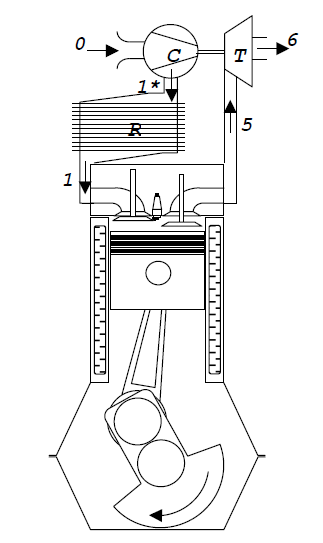
\includegraphics[scale=0.7]{img/Chap2_Q10.PNG}
  \caption{Montage d'un turbocompresseur}
  \label{Chap2_turbo}
\end{figure}


\subsection{Quels sont les intérets de la suralimentation ? expliquer les turbocompresseurs à géométrie variable et l'assitance électrique.}
\textbf{Intéret de la suralimention}: cf. Question \ref{Chap2Q10}.

\textbf{Turbo à géométrie variable + assistance électrique}: cf. CM4 slide 30, permet de fournir à l'admission la pression maximale acceptable par le moteur, et ce sur une plus grande plage de régimes de fonctionnement.

\subsection{Pourquoi la suralimentation et le downsizing sont indispensables dans un moteur moderne ?}
Avantages de la suralimentation repris à la Question \ref{Chap2Q10}. De plus, les moteurs compactes sont devenus indispensables actuellement dans le secteur de l'automobile.

\subsection{Moteur à Argon : intérêt et fonctionnement ? Pourquoi améliorer Gamma ? Pourquoi on a un faible taux de compression ?}
CM3 slides 5-6.

Dans le cas où on n'a pas spécialement accès à l'air ambiant, ou si on veut utiliser une réserve d'oxygène ne provenant pas de l'atmoshpère, on a intéret à changer le gaz diluant (d'habitude N2) par un autre pour augmenter le $\gamma$ du mélange (cf. Question \ref{chap1Q2}). L'argon est une bonne option ($\gamma=1.65$, au lieu de 1.4 pour N2).

Par contre, comme les capacités calorifiques diminuent, la température max atteinte est plus importante et on doit diminuer $\tau$ pour éviter tout risque de cliquetis (combustible gazeux dans l'exemple des slides).


\section{Aspects mécaniques et PME}

\subsection{Principales sources de frottement ?}
\label{Chap3Q1}
Il y a deux types de frottements :
\begin{itemize}
 \item Frottements secs: contact direct des organes en mouvement, imparfaitement séparés par un film mince de lubrifiant. Ex : segment-cylindre ou organes auxiliaires à faible vitesse de glissement.
 \item Frottements visqueux: lubrification hyrdodynamique, et donc interposition d'un film épais de lubrifiant. Ex : paliers, jupe du piston, et organes auxiliaires à vitesse de glissement élevée.
\end{itemize}

Les différentes sources de frottements considérées sont donc les suivantes:
\begin{itemize}
    \item Segments: pression de contact $p_s = p_{el} + p_g$, $p_g$ dépendant du moment dans le cycle, et uniquement considérée pour le premier segment. Expression (3.1) p. 47. Entre 80 kPa à 100 kPa. 
    \item Jupe du piston: expression (3.2) p. 50. Environ 30kPa.
    \item Embiellage et paliers: expression (3.3) p. 51. Environ 25kPa.
\end{itemize}

Finalement, $pmf$ peut etre réécrit sous la forme $$pmf = pmf_0 + k_s(2pmc+pmi) + k_v \cfrac{u}{D}$$

où (cf. syllabus p. 51):
\begin{itemize}
 \item $pmf_0$ est de l'ordre de \SI{100}{kPa} pour moteurs 4 temps, et \SI{50}{kPa} pour moteurs 2 temps.
 \item $k_s$ est de l'ordre de \SI{0.025}{}
 \item $k_v$ est de l'ordre de 1-\SI{1.5}{kPas} pour moteurs 4 temps, et \SI{0.5}{}-\SI{0.75}{kPas} pour moteurs 2 temps.
\end{itemize}


\subsection{Origines des sollicitations mécaniques dans un moteur monocylindre ? Comment les éviter dans un multicylindre ? Méthode de Lanchester ?}
Les sollicitations mécaniques viennent de la superposition de la pression équivalente d'inertie (externe, se transmet au niveau du support du moteur) et de la pression interne (ne sollicite que le bloc moteur car égalité de leur effet sur le piston et la culasse).  
Les forces d'inerties sont surtout importantes au PMH et PMB. Le travail résultant de ces forces est nul car il est symétrique sur l'entièreté du cycle. Par contre, la résultante des forces de pression n'est pas nulle (sinon pas de travail). 

Le couple induit par les forces d'inerties est plus que proportionnel à la vitesse de rotation. (au carré ?). Il y a des forces verticales et de rotation. 

Pour neutraliser les forces d'inertie d'ordre 1:
\begin{itemize}
 \item \textbf{Multicylindre}: déphaser les cylindres de $2\pi/n$, et du coup avoir un evenly timed firing sequence.
 \item \textbf{Monocylindre}: blancing shaft, cf. CM6 slide 23 et 27.
\end{itemize}

Pour neutraliser les forces d'inertie d'ordre 2 en multicylindre, on peut faire la même chose que pour H1 en monocylindre, mais en faisant tourner les balancing shaft à vitesse $2\omega$ et en adpatant les masses (méthode de Lanchester).




\subsection{Pourquoi on utilise Lanchester pour l'ordre deux et pas l'ordre 1 ?}
Parce que dans un multicylindre, l'ordre 1 est déjà compensé par le séquençage (evenly timed firing sequence). 


\subsection{Pourquoi les courbes de pmf en fonction de la vitesse du moteur ont une légère composante en carré ? (alors que les courbes théoriques sont linéaires)}
Au très grandes vitesses de rotation, on a un terme en $u^2$ qui devient important dans les frottements visqueux. {\color{red}pas sur, à vérifier!}


\subsection{L'intérêt d'un arbre à came variable ? Principe ?}
Permet de faire varier le timing d'ouverture/fermeture des soupapes (mais pas le temps d'ouverture). Arbre à came 3D, qu'on déplace de manière latérale. Intéret: optimiser les valve timing pour améliorer le rendement thermodynamique.

\subsection{Justifier l'ordre d'allumage des cylindres. Est-il toujours possible d'avoir un allumage régulier ?}
Pour lisser au mieux le couple généré par le moteur (du au cycle de la combustion et aux effet d'inertie), on répartit uniformément l'allumage des différents cylindres sur les 2 tours de vilebrequin qui forment le cycle complet. Cela permet de plus de supprimer les sollicitation d'ordre 1 pour les moteurs à au moins 2 cylindres.

Il est toujours possible d'obtenir un allumage régulier, à conditions de bien positionner les manetons sur le vilebrequin.

\section{Carburants et combustion}

\subsection{Pourquoi y a-t-il une température critique ? Est ce que la pression l'influence ? Les limites ?}
\label{Chap4Q1}
$T_c = T$ à laquelle le mélange peut s'auto-enflammer (= limite d'autoignition). Comme montré à la Figure \ref{img_chap4Q1} (courbe L), la limite d'auto-ignition est bien plus élevée pour les carburants légers que les carburants lourds. De plus, il est facile de l'atteindre avec des taux de compression modérés pour ces derniers. Elle est influencée par la pression, mais uniquement aux faibles valeurs de celle-ci. A partir de 10 bar, on peut considérer qu'elle n'a plus d'importance.

La température critique traduit la dépendance des mécanismes internes à la combustion envers la température (et la pression). En effet, la combustion est caractérisées par quatre réactions différentes:
\begin{itemize}
 \item \textbf{Initiation}: générations de radicaux à partir d'excitations externes.
 \item \textbf{Propagation}: 1 radical + 1 réactif = produit(s) + 1 radical
 \item \textbf{Ramification} (chain-branching): 1 radical + 1 réactif = produit(s) + X radicaux
 \item \textbf{Terminaison}: 1 radical + 1 réactif = produit(s)
\end{itemize}

La température critique est celle à laquelle toutes les réactions s'équilibrent pour maintenir constante la concentration des radicaux, et donc permettre la consommation des réactifs en produits à une vitesse stationnaire. Au delà de cette température (qui est elle-même influencée par les différentes réactions), le système réagit de façon explosive car génère plus de radicaux que ne consomme de réactifs. En-dessous, le système est inerte (cf. syllabus p. 70-74).

Notons finalement que la limite d'auto-ignition est fonction de la composition du mélange (cf. labo flamme en Essais de machine thermique).
\begin{figure}[H]
  \centering
  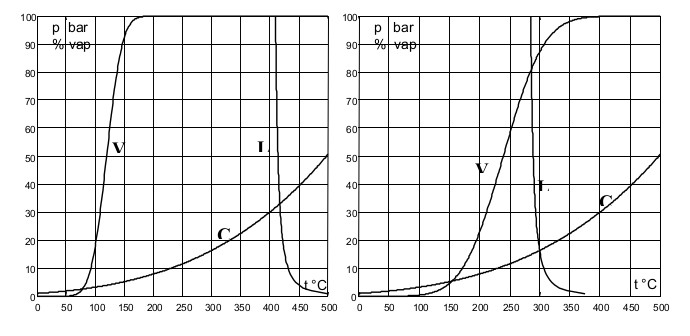
\includegraphics[width = 0.7\textwidth]{img/Chap4_Q1.jpg}
  \caption{Limite d'auto-ignition (L) et pression en fin de compression (C) dans le diagramme p-T pour des carburants légers (gauche) et lourds (droite). La fraction de vapeur aux différentes température (V) y est superposée.}
  \label{img_chap4Q1}
\end{figure}


\subsection{Quelles sont les types de transformations ? Expliquer les réactions radicalaires, et l'intérêt de les séparer.  }
Type de réactions radicalaires: cf. Question \ref{Chap4Q1}.

L'intéret de les séparer réside dans l'étude de leur dépendance à la température, pour en extraire la température critique d'auto-ignition d'un mélange. Pour se faire, il faut se baser sur l'équation d'Arrhénius pour obtenir les constantes de vitesse des différentes réactions. Elle fait intervenir différents facteurs, dont l'énergie d'activation et la fréquence des collisions.

Si plusieurs réactions de ramification ou de terminaisons sont possibles, les effets de pression peuvent s'équilibrer ou être exacerbés sur une petite plage. Il est donc important de les écrire séparément. Ce n'est pas toujours possible vu le nombre de réactions impliquées dans la combustion de l'ammoniaque par exemple. 


\subsection{Pourquoi n'est-ce pas intéressant de travailler à charge partielle ?}
Il faut bien distinguer les deux types de moteur sur leurs méthodes de réglage de la charge:
\begin{itemize}
 \item \textbf{Moteur SI}: richesse constante, on modifie le remplissage via une vanne papillon. Une charge partielle vient donc augmenter les pertes par pompage.
 \item \textbf{Moteur CI}: remplissage constant, on modifie la richesse à l'aide de la quantité de fuel injectée dans le cylindre. Un richesse trop faible voit son rendement de combustion diminuer, car température trop faible et beaucoup d'imbrulés proche des parois.
\end{itemize}
De plus, dans les deux cas les pertes mécaniques varient peu (cf. $pmf_0$ important par rapport à $pmf$), et ont donc une influence plus négative sur le rendement effectif à charge partielle qu'à pleine charge.

\section{Combustion dans les moteurs SI}
\subsection{Vitesse de flamme : valeur théorique, pratique, paramètres d'influence}
Flamme laminaire plane et stationnaire aux conditions standard de température et de pression: cf. Figure \ref{Chap3_v_flamme}. Max à 40cm/s pour $\phi=1$. Limites (cf. p83 syllabus) :  0.55 < $\phi$ < 2.5

En réalité, l'onde n'est ni plane (courbée dès la source, puis frippée par les turbulences) ni stationnaire (confinement).

Facteurs d'influence:
\begin{itemize}
 \item Richesse: cf. Figure \ref{Chap3_v_flamme}.
 \item Composition du carburant
 \item Turbulence: augmente la surface du front de flamme.
 \item Température et pression: si $T$ plus importante, plus de radicaux déjà présents et donc propagation plus rapide.
\end{itemize}

L'EGR influe donc sur la vitesse de flamme, car diminue la température à l'intérieur du cylindre.

En pratique, si on tourne a \SI{3000}{rpm}, avec $t_b =  \SI{5}{ms}$ (temps de combustion) et $D/2 = \SI{5}{cm}$, on a $c=\SI{0.05}{}/\SI{0.005}{} = \SI{10}{m/s}$ (cf. syllabus p. 89).

Une grande vitesse de propagation permet le design de moteurs SI avec de plus grands diamètres sans problème de cliquetis, pour peu que le coincement ne pose pas problème.

\begin{figure}[H]
 \centering
 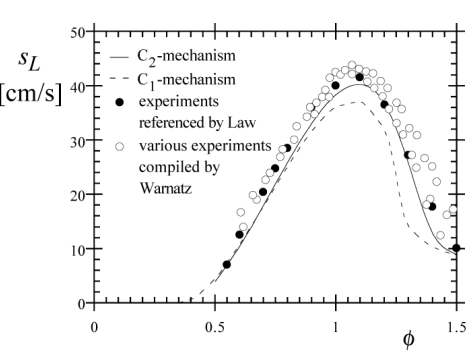
\includegraphics[width = 0.6\textwidth]{img/Chap3_vitesse_flamme.PNG}
 \caption{Vitesse de flamme laminaire du CH4}
 \label{Chap3_v_flamme}
\end{figure}


\subsection{Pourquoi travailler à richesse unitaire ?}
Plusieurs raisons:
\begin{itemize}
 \item Plusieurs zones intéressantes d'un point de vue polluants: $\phi \approx 0.65$ et $\phi \approx 1$ (cf. CM10 Slide 29).
 \item D'un point de vue puissance, plus intéressant $\phi \approx 1$ (cf. Fig. 5.7 p. 97). Combustion imparfaite en $\phi = 1$, mais
  \begin{itemize}
    \item $pmi$ max pour $\phi = 1.1$, mais au prix d'une forte surconsommation pour un faible gain de puissance
    \item $\eta_C$ max pour $\phi = 0.85$, mais forte perte de puissance pour un faible gain en rendement
  \end{itemize}
 \item $\phi>0.6$ pour permettre une vitesse de flamme suffisante, et donc assurer une bonne propagation
\end{itemize}

$\phi = 1$ est donc l'optimum pour les applications automobiles qui ont des besoins de compacité et fortement soumises à des controles de pollution.


\subsection{Quelles sont les sources d'imbrulés ?}
2 possibilités:
\begin{itemize}
 \item Coincement de la combustion (mauvaise propagation), à cause d'une température trop faible proche des parois (peut-être lié à une trop faible richesse).
 \item Excès de carburant ($\phi$ > 1) qui donne une combustion incomplète. 
\end{itemize}


\subsection{Expliquer le graphe pmi - richesse (fig 5.7 du syllabus)}
La Figure \ref{img_chap5Q4} reprend l'évolution de $pmi$ en fonction de la richesse du mélange, ainsi que son approximation linéaire pour les zones pauvre et riche. Les équations de ces droites sont obtenues p. 95-96 du syllabus, en développant la réaction chimique avec tous les produits possibles.

La courbe réelle s'écarte nettement de ces prédictions théoriques, essentiellement pour des mélanges très pauvres et très riches. Cela est du à une combustion imparfaite pour les mélanges très pauvres du fait d'une vitesse de flamme faible et de parois relativement froides qui empechent le bon déroulement de la réaction dans ces zones. Les mélanges très riches souffrent quant à eux du même mal, mais du cette fois-ci à une trop faible concentration en oxygène qui ne permet pas partout la combustion.

Finalement, les écarts observés sous le point d'intersection des deux droites est du à des richesses locales $\phi_{loc}$ déviant de la valeur moyenne $\phi$. Certaines zones présentent en effet des richesses locales $\phi_{loc}>1$ alors même que $\phi<1$, menant à des combustions incomplètes. Le maximum de $pmi$ est enfin observé lorsque $\phi_{loc}\geqslant 1$ partout dans le cylindre.
\begin{figure}[H]
  \centering
  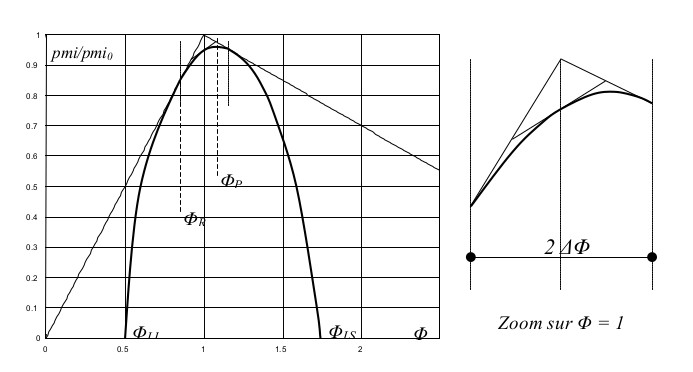
\includegraphics[width = 0.7\textwidth]{img/Chap5_pmi_phi.jpg}
  \caption{Influence de la richesse sur pmi.}
  \label{img_chap5Q4}
\end{figure}

\subsection{Quelles sont les raisons qui conduisent à un ratage à l'allumage ?}
Pour que l'étincelle engendre une flamme qui se propage, il faut que le flux de chaleur dégagé par la combustion soit plus grand que le flux conductif à la périphérie. De cela résulte une taille critique de noyau d'ignition. Il y a donc une double exigence (cf. syllabus p. 85-86):
\begin{itemize}
  \item Densité d'énergie suffisante, c'est à dire $T_f$ que doit atteindre le noyau d'allumage.
  \item Quantité d'énergie suffisante, c'est à dire diamètre critique $d_c$.
\end{itemize}

Les paramètres qui influencent cela sont:
\begin{itemize}
    \item EGR : trop de recirculation diminue la température et $\phi$.
    \item Avance à l'allumage : si on déclenche l'étincelle trop tot, la compression n'est pas à son maximum et donc la température est trop faible. 
    \item La richesse du mélange autour de la bougie : si la dilution est trop importante la flamme ne prendra pas. C'est pourquoi on travaille avec une charge stratifiée par exemple (ou une pré-chambre).
\end{itemize}
   


\subsection{Expliquer la combustion dans un moteur à essence. Intéret de la charge stratifiée ?}
Cela permet d'avoir une richesse plus élevée proche de la bougie (meilleure propagation au départ) et moins élevée proche des parois (moins d'imbrulés et de pertes pariétales).


\subsection{Expliquer le cliquetis. Comment l'éviter ? }
Le cliquetis est causé par l'auto-ignition du mélange dans un moteur SI. Ce phénomène est loin d'etre voulu, car engendre:
\begin{itemize}
 \item Des ondes de pressions intenses dans la bande 3-10kHz.
 \item Des vitesses locales très élevées atteintes par les gaz brulés, entrainant une forte augmentation de $\epsilon_P$ (et donc diminution du rendement).
 \item Une destruction plus ou moins sévère des parois les moins bien refroidies.
\end{itemize}

Il apparait une fois la température critique $T_c$ atteinte depuis un délais $\delta$ supérieur au délais d'auto-ignition (cf. Fig. 5.5 p. 91). Comme la température lors de la combustion monte toujours plus haut que $T_c$, il s'agit d'une course entre la vitesse de flamme et le délai d'auto-ignition. Si la flamme a tout brulé avant le délais, il n'y a pas de cliquetis. Pour l'éviter, on doit donc jouer sur les paramètres de combustion pour réduire le temps de propagation de la flamme, et/ou augmenter le délais d'auto-ignition du mélange (cf. syllabus p. 93-94).

\textbf{Temps de propagation de la flamme}
\begin{itemize}
 \item Forme et dimensions de la chambre de combustion.
 \item Développement de turbulences pour augmenter la vitesse de flamme par transport de matière.
 \item $\phi$ qui donne une vitesse de flamme maximale proche de la stoechiométrie. Attention que ce paramètre influence également le délais d'auto-ignition.
\end{itemize}

\textbf{Délais d'auto-ignition du mélange}
\begin{itemize}
 \item $\tau$, $p_1$, $T_1$, $\phi$, angle d'allumage qui déterminent la sévérité des conditions dans le cylindre, et donc le moment auquel $T_c$ est atteinte.
 \item Nature du carburant $\rightarrow$ indice d'octone (RON et MON) pour les combustibles liquides et indice de méthane pour les combustibles gazeux (cf. syllabus p. 94-95).
\end{itemize}

\textbf{Notes}
\begin{itemize}
  \item Le rendement thermique est d'autant plus élevé qu'on est proche des conditions de cliquetis (car température élevée).
  \item Le cliquetis ne pose pas de problème majeur en moteur CI, cf. syllabus p. 108.
\end{itemize}



\subsection{Indice d'Octane et de Cétane ? Lien entre les deux ? Qu'est-ce qu'un bon carburant ?}
\paragraph{Indice d'Octane (carburant liquide, moteur SI)} Il s'agit d'un étalonnement des carburants entre l'iso-octane d'indice 100, et l'heptane 
d'indice 0. 2 types: RON (research) et MON (motor). Il est calculé avec le moteur CFR. Valeurs usuelles du RON : 95, 98. MON 5 points plus bas. Un haut indice d'octane ne forme que lentement des radicaux et augmente donc le délai d'auto-ignition. Pour un haut indice il faut des chaines courtes, ramifiées, des insaturés et des composés cycliques. 

\paragraph{Indice de Méthane (carburant gazeux, moteur SI)} 100 pour CH\textsubscript{4}, 0 pour H\textsubscript{2}. Le plus haut est le moins auto-inflammable. Echelle très sensible. On calcule tant des valeurs d'indice de méthane que d'octane pour certains carburants gazeux.. quid?

\paragraph{Indice de Cétane, (moteur CI)} 100 pour le cétane (s'enflamme facilement), 0 pour le méthylnaphtalène (s'enflamme difficilement). Valeurs classiques: 40 pour les fuels lourds, 50 pour les petits moteurs. Les paramètres favorables sont : des chaines longues, rectilignes, saturées et non cycliques.

Donc en gros comme les objectifs sont opposés pour l'essence et le diesel, les indices de cétane et d'octane sont aussi opposés. Un bon indice d'Octane implique un indice de Cétane très bas. 

\subsection{Expliquer l'EGR. Sous quelles conditions l'utilise t-on ? Différence entre moteur à essence et diesel ?}
Réinjection de fumée d'échappement directement dans le cylindre (après une phase potentielle de refroidissement). Pour les moteurs SI (CM11 slides 12-16):

\textbf{Avantages}
\begin{itemize}
  \item Moins de pertes pompage à charge partielle (vanne papillon reste plus ouverte, puisque on gère le remlissage par ajout de fumées).
  \item Plus grande capacité thermique, et donc plus faible T max.
  \item N'affecte pas le catalyseur 3 voies
  \item Impact positif sur les polluants
\end{itemize}

\textbf{Inconvénients}
\begin{itemize}
  \item Augmente le travail de compression (mais aussi le travail d'expansion)
  \item Affecte fortement la propagation de la flamme. C'est pourquoi on doit le limiter à 15\% max.
\end{itemize}

Dans le cas des moteurs CI, on n'a plus l'intéret de la limitation des pertes par pompage (pas de vanne papillon). Il a tendance à augmenter la richesse (pour une quantité de fuel injectée inchangée). Au niveau des polluants: cf. CM11 slide 76-77 + notes de cours CM12. Ca diminue essentiellement la concentration en NOx, tout en augmentant la taille des suies produites (qui sont donc plus faciles filtrer).


\subsection{Dilution par air pour par EGR ? Différence entre les deux ?}
CM11 slide 15: le rendement est plus augmenté avec une dilution à l'air, mais on ne profite alors pas de l'impact positif de l'EGR sur les polluants (ça a même un effet négatif puisque plus grande production de NOx).

\subsection{Quels polluants dans un moteur à essence ?}
\begin{itemize}
    \item CO: En mélange riche car il est le résultat d'une combustion en manque d'oxygène. Hautement toxique. 
    \item NOx: C'est le principal problème. D'autant plus abondant que la température est élevée et qu'il y a d'oxygène disponible (donc pic en richesse juste substoechimétrique, car si $\phi<<1$ T trop basse), là où les autres sont limités et le rendement meilleur.
    \item COV (composés organiques volatils): constitués d'hydrocarbures (HC) et d'aldéhydes. Proviennent du coincement de la flamme (température trop faible, ou richesse trop faible ou trop haute). Engendrent la formation d'ozone et de PAN (peroxyacetyl nitrate), cf CM10 slides 21-22).
\end{itemize}

\subsection{NOx dans les diesels et essence. Quelles paramètres pour les diminuer ?}
Les NOx sont produits par oxydation de l'azote. Cette réaction est donc favorisée à haute température, et forte concentration d'oxygène.

\textbf{Dans les moteurs SI}, ils sont donc le plus abondant à richesse juste sub-stoechiométrique. Pour les limiter, on pourrait travailler à plus faible ou plus forte richesse (cf. Fig 5.8 p. 100). Seulement, une richesse élevée induirait un gaspillage de carburant ainsi que d'autres polluants liés à la combustion incomplète. La zone de travail à faible richesse est exploitée dans certaines applications stationnaires, mais présente une faible densité énergétique du fait du faible $\phi$.

\textbf{Dans les moteurs CI}, le NO est produit dans les zones pauvres en bordure de stoechiométrie, qui existent autour de chaque noyau de combustion. La teneur en NO dans les gaz d'échappement est donc quasi-proportionelle à la charge du moteur. Une manière de la limiter est d'utiliser une injection indirecte car favorise le brassage des espèces dans le cylindre, uniformise donc les zones de combustion et en abaisse les températures de pointe.

\textbf{Dans les deux types de moteurs}, il est possible de réduire la production de NOx par utilisation de l'EGR. Au final, il s'agit d'optimiser les paramètres de conception et d'utilisation pour maximiser les rendement et la puissance tout en limitant les émissions (-> cartographie).

\textbf{Deux possibilités pour traiter} les NOx après la combustion:
\begin{itemize}
 \item Three-way catalytic converter (Moteur SI, CM10 slides 33-34).
 \item Selective Catalytic Conversion (SCR): on ajoute de l'amoniac pour réduire les NOx (CM10 slide 33-34 et CM11 slide 79).
\end{itemize}

\subsection{Utilité de la sonde Lambda ?}
La sonde lambda permet de détecter si un mélange est riche ou pauvre, car son signal évolue très vite dans la zone proche de $\phi=1$ (cf. Figure \ref{img_Chap5Q13_lambda}, tirée des slides de Essais de machines thermiques). Elle est très pratique dans l'application du three-way catalyst, qui nécessite une richesse très proche de 1 pour fonctionner de manière optimale (cf. CM10 slide 35). On peut donc l'utiliser comme boucle de controle sur la richesse du mélange pour favorisant l'action du pot catalytique.

\begin{figure}[H]
  \centering
  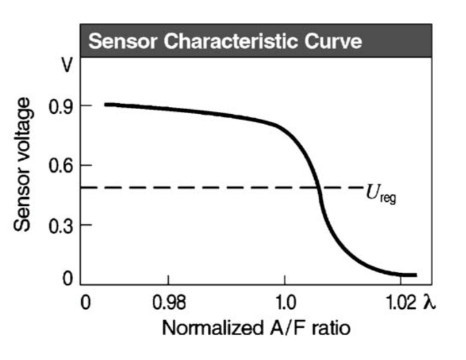
\includegraphics[width = 0.4\textwidth]{img/Chap5_lambda.jpg}
  \caption{Signal renvoyé par la sonde lambda en fonction de l'excès d'air.}
  \label{img_Chap5Q13_lambda}
\end{figure}


\subsection{Peut-on diminuer la charge tant qu'on veut dans un moteur à essence ?}
Il faut s'assurer que la combustion ait bien toujours lieux pour que le moteur continue à tourner, même à vide. Pour cela, il s'agit d'assurer une richesse minimale du mélange air/carburant lorsque le moteur fonctionne au ralenti. $\phi$ ne peut en effet descendre en dessous de 0.6, pour que la flamme puisse se propager suffisament.

\section{Combustion dans les moteurs Diesel}
\subsection{Expliquer le cognement. Comment l'éviter ? Pourquoi la giration ?}
La combustion en moteur CI est séparée en trois phases (cf. Fig 6.1 p. 104):
\begin{enumerate}
 \item Le délais à l'auto-ignition
 \item La combustion rapide
 \item La combustion lente
\end{enumerate}

Lors de la phse de combustion rapide, la pression monte brutalement produisant un bruit de cognement, ou diesel knock. Notons que ce phénomène est assez similaire au cliquetis des moteurs SI, mais n'est cependant pas très grave car:
\begin{itemize}
 \item Fluide plus froid, et donc fréquence plus basse
 \item Pas d'effet thermique destructeur sur les parois de la chambre (en contact avec de l'air plutot que des gaz comburés).
\end{itemize}

Il induit tout de même un bruit important, qu'on essaie de limiter. Pour ce faire, on peut:
\begin{itemize}
 \item Injection en plusieurs parties, pour qu'une première quantité de carburant brule avant que la suite ne soit injectée. Cela a pour effet d'échelonner la montée en pression dans le cylindre. Cela peut aussi etre par une injection à débit variable (cf. injecteur à teton).
 \item Une bonne dipersion du carburant dans la chambre. Il faut tout de même faire attention que le mélange soit inflammable, surtout dans le cas d'injections multiples.
 \item Pulvériser finement.
 \item Petits moteurs plus sujet au cognement, car généralement injection en une seule fois.
 \item Injection indirecte: permet l'utilisation d'injecteur à un seul trou ou à teton, et confine le cognement dans une zone statique qu'il est plus facilement possible d'isoler accoustiquement.
 \item Indice de cétane élevé (car mélange d'autant plus explosif que le délais est grand, cf. début p. 108). Cependant, il faut une adéquation entre moteur et fuel: petits moteurs, il faut un fuel plus léger à grand indice de cétane pour ne pas que des gouttes atteignent les parois, alors que les gros moteurs lents peuvent utiliser des fuels plus visqueux, à indice de cétane assez bas pour éviter la formation de cénosphères (craquage thermique de gouttes non évaporées).
\end{itemize}

La giration a un effet de dispersion et mélange homogène des composés. Elle a donc tendance à répartir la charge, et à diminuer le cognement.


\subsection{Polluants du Diesel ? + méthode pour les éliminer}
Cf. syllabus p. 119-120.

\textbf{Particulate matter (PM)}: suies formées en zones chaudes et riches, et les cénosphères issues du craquage thermique des gouttes de carburant non encore évaporées. Solution: filtre à particules + élévation de la température pour en provoquer l'oxydation au contact de l'oxygène résiduel des fumées d'échappement.

\textbf{NOx}: produit en zone pauvre, en bordure de stoechiométrie donc quasi proportionnel à la charge du moteur. Solution: 
\begin{itemize}
 \item Injection indirecte: favorise le brassage des espèces dans le cylindre, uniformise donc les zones de combustion et en abaisse les températures de pointe.
 \item EGR
 \item Lean-NOx Trap (LNT) et Diesel Oxydation catalyst: on chauffe pour transformer le NO en NO2 (CM11 slides 78-80).
 \item Selective Catalytic Conversion (SCR): on ajoute de l'amoniac pour réduire les NOx (CM10 slide 33-34 et CM11 slide 79).
\end{itemize}

\textbf{Hydrocarbures (HC)}: zones trop pauvres ou trop froides, typiquement au démarrage au après une longue période charge partielle. Solution: pot catalytique d'oxydation (principalement à base de Pt/Rh).

\textbf{CO}: formation dans les zones en déficit d'oxygène, et lors du phénomène de coincement (mélange partout trop pauvre ou trop froid). Solution: filtre à particule + température (comme pour PM).

\textbf{SO2}: oxydation du soufre, si il y en a. Solution: on l'enlève du fuel à la source.


\subsection{Evaporation d'une goutte (chimique et physique). Se servir d'un graphe}
Cf. Fig. 6.3 p. 107. Le fuel est injecté sous haute pression, et se disloque donc en brouillard dès son entrée dans la chambre. Avant l'enclenchement de la combustion (et délais d'auto-ignition), il faut qu'il s'évapore. Le temps nécessaire à cela peut etre divisé en deux parties: le délais de chauffage pour atteindre la température d'évaporation, puis le délais nécessaire à cette évaporation. La température n'évolue plus dans cette seconde phase (évaporation), mais peut encore monter après pour atteindre la température critique d'auto-ignition.

Les équations (6.1) et (6.3) donnent les bilans thermiques liés au chauffage et à l'évaporation, et les Eq. (6.2) et (6.4) les délais correspondants.

\subsection{Intérêt de l'injection directe et indirecte ?}
Cf. syllabus p115-119

\textbf{Directe}: L'injecteur amène le carburant directement dans la chambre de combustion.
\begin{itemize}
 \item Meilleur rendement (car moins de pertes pariétales)
 \item Inconvénients: cf. syllabus p. 118-119.
\end{itemize}

\textbf{Indirecte} : 
\begin{itemize}
 \item Pression d'injection plus basse => moins technologique, plus facile et moins chère.
 \item Pose peu de problèmes de mise au point.
 \item Moins de cognement (confiné dans une zone statique).
 \item Utilisation d'injecteur à un trou ou à téton (faible risque d'obstruction).
 \item Inconvénient: défavorable au rendement thermique du moteur (augmentation de $\epsilon_P$).
 \item $\rightarrow$ moteurs de petite taille, pour lesquels injection directe serait chère, et pas grave d'avoir un moins bon rendement.
\end{itemize}

\section{Respiration et remplissage}

\subsection{Quand est-il utile d'ouvrir les différentes soupapes ? Avantages et inconvénients des anticipations et retards}
CM7 Slides 24-28
\begin{itemize}
 \item EVO: trade-off entre travail d'expansion et de pompage
 \item EVC: internal EGR et inertie
 \item ICO: internal EGR et homogénéisation du mélange
 \item IVC: remplissage et inertie
\end{itemize}


\subsection{Qu'est ce qui dicte la dimension des soupapes ?}
CM7 slides 9-11 et 17-18.

Expression du remplissage en fonction de $\Delta a$ et $\Delta e$
\begin{itemize}
 \item Intéret à plus diminuer $\Delta a$ car multiplié par $\tau$
 \item Donc on met plus d'inlet valves que d'exhaust
\end{itemize}

Niveau taille, on impose le même pressure drop, et donc inlet valves plus grandes en surface:
$$\cfrac{A_a}{A_e} = \sqrt{\cfrac{T_e}{T_a}} $$


\subsection{Comment adapter les ouvertures en fonction du régime où on se trouve ?}
Par un système de contrôle de valve fonction du régime (Variable Valve Timing). Essentiellement 2 possibilités:
\begin{itemize}
 \item Arbres à cames 3D
 \item Soupapes controlées electroniquement
\end{itemize}


\subsection{Qu'est ce qui est le mieux pour le remplissage : turbocharger ou supercharger ?}
\textbf{Turbocharger}: réutilise les gaz d'échappements (énergie normalement perdue) pour augmenter le remplissage, donc meilleur rendement.

\textbf{Supercharger}: utiliser de la puissance mécanique pour augmenter le remplissage. Ne réutilise donc pas les gaz d'échappement. Moins bon rendement, mais beaucoup plus réactif.


\subsection{Qu'est ce qui influence le remplissage dans un moteur 4 temps ?}
C'est surtout le taux de compression et les pressions d'admission et d'échappement qui dictent le rempolissage:
$$ r=\frac{\tau(1-\Delta a) - (1+\Delta e)}{\tau -1} $$

Ces paramètres sont influencés par (cf. CM7 slide 6):
\begin{itemize}
    \item Valve timing
    \item Suralimentation ou non
    \item Carburant et son type d'injection (directe/indirecte)
    \item Température d'admission
    \item RPM et charge
    \item Géométrie du moteur : valves,tuyaux, tête de piston,...
\end{itemize}

\subsection{Comment s'effectue le remplissage d'un moteur 2 temps ? Quels sont les problèmes liés ?}
Le remplissage se fait par balayage transversal ou longitudinal $\rightarrow$ schéma CM7 slide 40
\begin{itemize}
 \item Transversal : La vanne de sortie se trouve opposée à l'entrée, à même hauteur
 \item Longitudinal : sortie sur le haut
\end{itemize}

L'air est en mouvement quand les vannes d'entrées et de sorties sont ouvertes en même temps. Car le temps de respiration est bien plus court que pour un moteur 4 temps. En pratique, on ouvre la sortie puis l'entrée, avant de fermer l'entrée puis la sortie.

Le problème vient d'une perte quasi irreductible de carburant, qui s'échappe directement sans parcourir le cycle (de l'ordre de 20\%). Ca plafonne donc $pme$ des moteurs deux temps (car limitation du remplissage pour ne pas perdre trop de fuel)  à 75\% de la valeur des moteurs 4 temps pour la même cylindrée, et limite donc l'avantage en puissance spécifique des moteurs 2 temps à 1.5 (au lieu de 2).

Les moteurs diesel 2 temps ne connaissent pas ce problème, car injection du carburant après (ou à la fin de) la phase de respiration.



\subsection{Qu'est ce que l'indice de Mach ? }
Cf. CM7 slide 16. De base, le nombre de Mach est défini comme le rapport entre la vitesse d'un fluide et celle du son. Ici, on connait la vitesse du piston $u$, du coup par conservation de la masse et sans considérer de variation de la masse volumique on a:
\begin{eqnarray*}
  Z	&=& \cfrac{\cfrac{\pi D^2}{4}}{A}\cdot \cfrac{u}{c_0}
\end{eqnarray*}
Avec $A$ la surface de passage du fluide à travers les soupapes, et $c_0 = \sqrt{\gamma R^*T}$ la vitesse du son. Pour avoir un grand remplissage, il faut garder Z<\SI{0.6}{}.






\subsection{Pourquoi injecter de l'eau à l'entrée (BMW) ?}
Ca permet d'abaisser la température dans le cylindre, par évaporation de l'eau lors de la combustion. Les avantages sont multiples:
\begin{itemize}
 \item Réduire le risque de cliquetis
 \item Permettre des taux de compression plus élevés, car cliquetis réduit
 \item Réduction des émissions de NO, car température plus faible
\end{itemize}

C'est du coup vachement cool, mais doit etre utilisé avec précautions (pas tout le temps) et faire partie de l'optimisation de la carto, car ses effets sont néfastes à faible charge où la diminution de la température peut mener au phénomène de coincement et de combustion incomplète.

Sources
\begin{itemize}
 \item \url{http://newatlas.com/bmw-water-injection-efficiency-power/38289/}
 \item \url{https://en.wikipedia.org/wiki/Water_injection_(engine)}
\end{itemize}


\section{HCCI}

\subsection{Fonctionnement et contrôle d'un moteur HCCI ? Quelle zone de fonctionnement (richesse) ?}
HCCI: Homogeneous Charge Compression Ignition. Le concept lie moteur SI et CI: on brule un mélange gazeux homogène, à allumage par compression. Du coup, on doit imposer faible richesse et faible température pour ne pas détruire le moteur (knock en moteur SI classique) (cf. Figure \ref{chap8_phi_T}).
\begin{figure}[H]
 \centering
 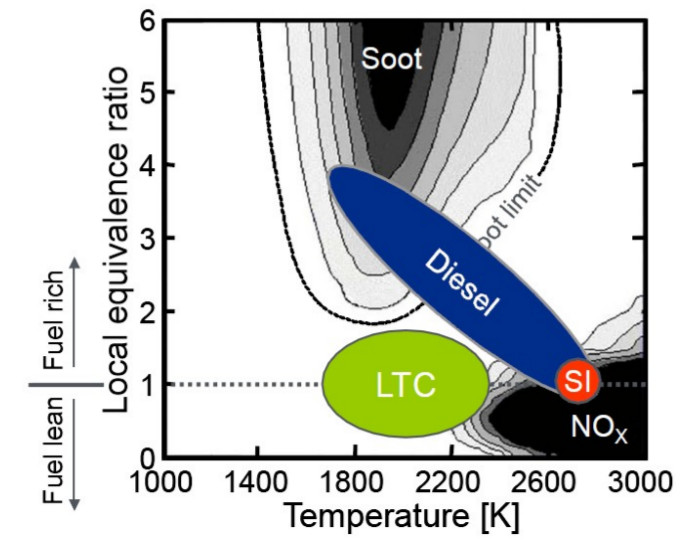
\includegraphics[width = 0.5\textwidth]{img/Chap8_phi_T.jpg}
 \caption{Types de combustions dans un diagramme $\phi$-T}
 \label{chap8_phi_T}
\end{figure}


Pour ce faire, le fuel doit etre prémélangé à l'air lors de son introduction dans le cylindre. On n'a donc aucun controle direct sur le début de la combustion (d'habitude, étincelle en SI et timing d'injection du fuel en CI). Pourtant, le timing de combustion est déterminant au niveau du travail développé et donc du rendement du moteur. On doit donc trouver d'autres manières de controler cette combustion.

Le problème, c'est que les paramètres l'influençant sont très (très!) nombreux. De plus, les plages de valeurs autorisées pour les différents paramètres assurant le bon fonctionnement du moteur sont assez restreintes. Cela en fait donc un moteur à la fois difficilement controlable, et peu flexible.

Paramètres de controle (cf. Séminaire HCCI slide 15):
\begin{itemize}
 \item Wall temperature
 \item $\tau$
 \item Charge distribution
 \item EGR
 \item Air temperature
 \item Injection timing
 \item EGR temperature
 \item Valve timing
 \item $\phi$
 \item Inlet pressure
 \item Fuel composition
 \item Engine speed
\end{itemize}

Richesse: doit etre comprise entre \SI{0.28}{} (pour $\eta_c$) et \SI{0.31}{} (pour réduire les NOx) (cf. Séminaire HCCI slide 49).



\subsection{D'où viennent les hydrocarbures imbrulés et le CO ?}
Zones à trop froides ou à trop faible richesse locale.


\subsection{Quel type de combustion a une vitesse de flamme qui joue sur la combustion ?}
\begin{itemize}
 \item Pas HCCI (ni diesel) : tout brule en même temps
 \item Pas PPC (partially premixed combustion)
 \item PCC (pre-combustion chamber) : OUI
 \item DISI : direct injection spark ignition : OUI
\end{itemize}
En somme tout ce qui est SI.


\section{Cartographies}
\begin{eqnarray*}
  pme	&=& M_e\cdot\cfrac{t\pi}{V_c}\\
	&=& \eta_e\cdot\cfrac{m_cPCI}{V_c}\\
  c_s	&=& \cfrac{1}{\eta_ePCI}
\end{eqnarray*}

Donc étudier $pme$, $M_e$, $\eta_e$ ou $c_s$ est strictement équivalent, il y a juste un facteur de proportionnalité entre toutes ces valeurs.

\subsection{Tracer les courbes couple/vitesse (pour moteurs SI et CI, avec et sans turbo}
Normalement, $pmi$ n'est pas fonction de la vitesse de rotation. $pme$ est alors une droite décroissante car $pmf$ est fonction de $\omega$.
\begin{itemize}
 \item A grande vitesse de rotation, le travail de pompage augmente signigicativement et limite donc le couple max.
 \item A faible charge, le travail de pompage augmente fortement pour le moteur SI, à cause de la vanne papillon. En plus, on diminue $r$ donc $\eta_{ti}$ diminue.
 \item Ce n'est pas le cas pour le moteur CI. Dans les deux cas, la consommation spécifique est très élevée car le fuel sert essentiellement à vaincre $pmf$.
 \item A faible vitesse de rotation, $\epsilon_P$ augmente et vient limiter $\eta_{ti}$ et donc le couple. Ce phénomène est plus important en moteur CI, car $\tau$ plus grand.
 \item Le turbo vient augmenter le remplissage. On peut donc diminuer $\phi$. Ca a pour conséquence d'améliorer $\eta_ti$ par diminution de $\phi$ (influence sur l'exposant $x$), et diminution des pertes partiétales par augmentation de r. De plus $pmi$ augmente (car $r$ augmente). Donc au final, plus grand couple et meilleur rendement.
\end{itemize}


\subsection{Consommation d'un moteur essence en fonction de la charge. Pourquoi ?}
La charge est définie comme le rapport entre $pme$ et $pme_N$ à la vitesse considérée (cf. syllabus p. 56). Il s'agit de clarifier ce qu'on entend par consommation: consommation spécifique $c_s$ ou consommation nette $\dot{m}_c$?

Pour peu qu'on reste dans des limites où $\eta_{ind}$ reste constant, $pmi$ est directement proportionnelle à la charge (prop à $r$). $pmf$ vient juste décaler la courbe. Limites:
\begin{itemize}
 \item $pmf$ a un facteur prop à la charge
 \item $\eta_{ind}$ diminue fort pour de très petites valeurs de charge, car phénomène de coincement (zones trop pauvres et/ou trop froides) qui détruisent le rendement de combustion $\eta_c$.
 \item La charge max est atteinte pour une richesse un peu supérieure à 1 (cf. Fig. 5.7 p. 97), qui mène à une forte augmentation de la consommation pour un faible gain en $pmi$, et donc une diminution du rendement et une augmentation de la consommation spécifique.
\end{itemize}


\subsection{Savoir justifier les formes des cartographies des polluants}
\textbf{Moteur SI}: Influence de $\phi$ sur les polluants CM10 slide 29.
  \begin{itemize}
   \item CO: augmente très fort si richesse augmente -> varie peu, car richesse ne dépasse normalement jamais 1.
   \item NOx: diminue très fort si richesse diminue -> très influencé par l'EGR
  \end{itemize}

\textbf{Moteur CI}
  \begin{itemize}
   \item CO: Production en zone pauvre et/ou froide, donc beaucoup plus à faible charge.
   \item NOx: produit en zone pauvre, en bordure de stoechiométrie donc production quasi proportionnelle à la charge. Mais du coup aussi fortement influencé par l'EGR: si fort EGR, moins de zones en bordure de stoechiométrie et donc moins de NOx.
  \end{itemize}


\end{document}
